\section{The rules on the characters}
\label{sec:characters}

Table~\ref{tab:characters} gives exact recall of the 18 characters, with each rule applied to the whole set. Each recall cell is the mean number recalled over 200 draws, with the range in parentheses when it varies. The test and 20\% columns use the committed query files, so only the update order of the classical rules varies. The fresh columns draw new noise too. The intervals given in the text for these means are Monte Carlo error on one fixed set of patterns and say nothing about other pattern sets.

\begin{table}[t]
\caption{Exact recall of the 18 characters (of 18): mean over 200 draws, with the range in parentheses when it varies, and, in the last column, the number of the 18 characters that are fixed points (for the modern network, that come back unchanged from a clean query). Storkey uses the file order of the patterns.}
\label{tab:characters}
\centering
\scriptsize
\setlength{\tabcolsep}{3pt}
\begin{tabular}{@{}lccccc@{}}
\toprule
Rule & Test file & 20\% file & Fresh 10\% & Fresh 20\% & Fixed \\
\midrule
Hebbian & 0 & 0 & 0 & 0 & 0 \\
Hebbian, 0/1 update & 0 & 0 & 0 & 0 & 0 \\
Storkey & 3 & 2.93 (2--3) & 3 & 2.91 (2--3) & 3 \\
Covariance & 0 & 0 & 0 & 0 & 0 \\
Pseudoinverse & 18 & 13.78 (10--18) & 17.22 (15--18) & 13.32 (8--18) & 18 \\
Modern, $\beta=4$ & 0 & 0 & 0 & 0 & 0 \\
Modern, $\beta=16$ & 14 & 13 & 13.19 (12--14) & 12.74 (10--14) & 14 \\
Modern, $\beta=64$ & 18 & 18 & 17.93 (16--18) & 17.57 (15--18) & 18 \\
Nearest pattern & 18 & 18 & 17.94 (16--18) & 17.56 (15--18) & 18 \\
\bottomrule
\end{tabular}

\end{table}

Hebbian storage, the 0/1 update, the covariance rule, and the modern network at $\beta = 4$ recall none of the characters from any query set, and none of the 18 is a fixed point. The pseudoinverse rule makes all 18 characters fixed points and recalls all 18 from the test file in all 200 update orders. On the 20\% file, though, it recalls \N{f:valid42:pinv:mean} of 18 on average [\N{f:valid42:pinv:lo}, \N{f:valid42:pinv:hi}], anywhere from \N{f:valid42:pinv:min} to \N{f:valid42:pinv:max} across the 200 orders, and all 18 in only \N{g:pinv_all18_pct}\% of orders (Fig.~\ref{fig:spread}). The 17 of 18 reported in the original submission was a lucky draw: \N{g:pinv_ge17_n} of the 200 orders (\N{g:pinv_ge17_pct}\%) reach 17 or more. The rule makes stored patterns fixed points except in rare, nearly identical sets (in \N{pfx:bad} of the \N{pfx:total} synthetic networks, all at $\rho \ge \N{pfx:minlevel}$, at least one stored pattern is not, because some unit's weights are zero in exact arithmetic, and the code sets them to exactly zero, so the tie rule sets that unit to $+1$), and it does not make their basins wide enough for 20\% noise.

\begin{figure}[t]
\centering
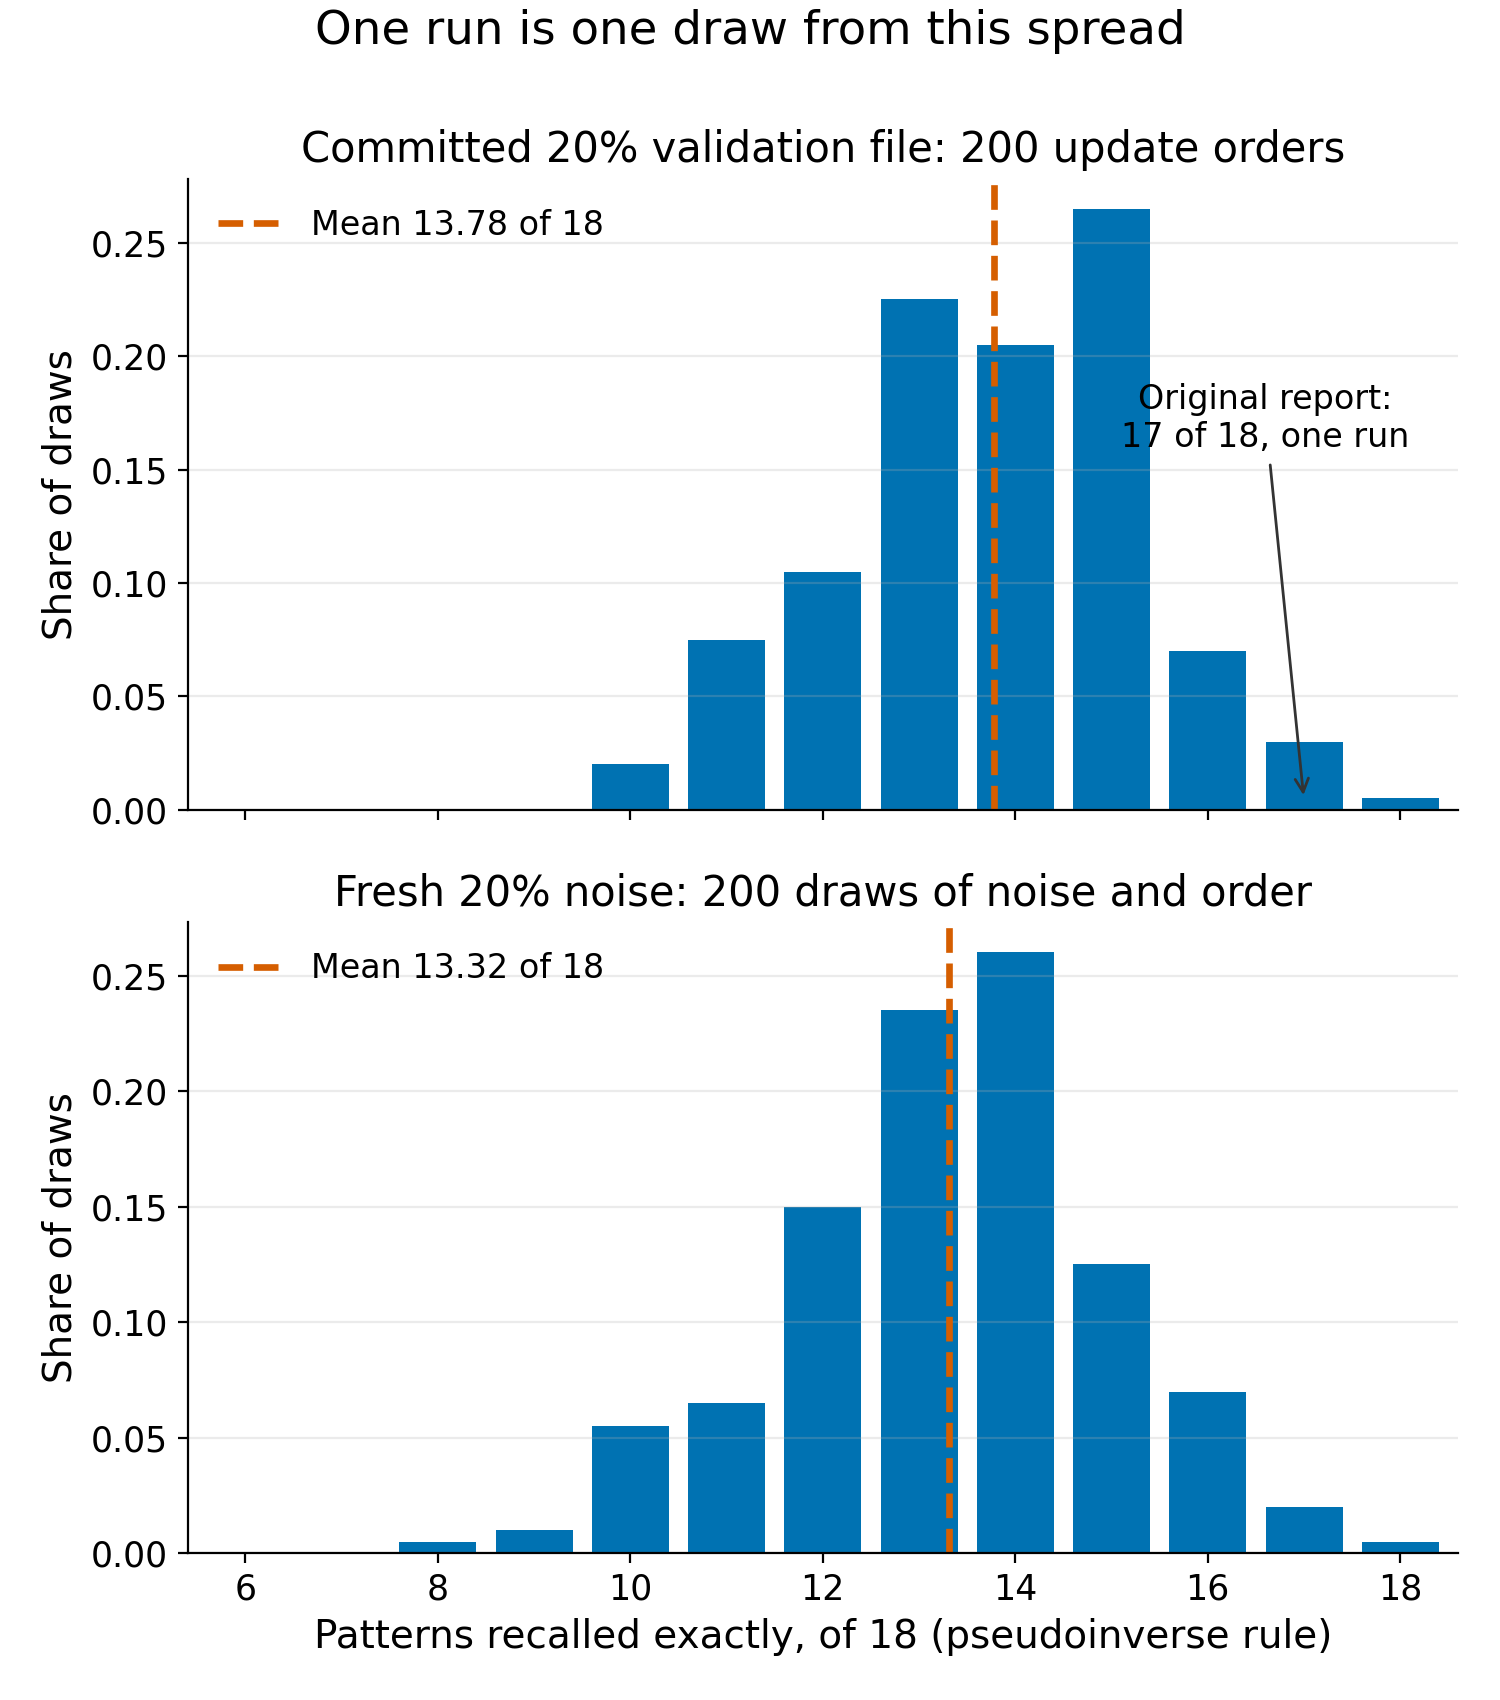
\includegraphics[width=\columnwidth]{../study/figures/fig5_pseudoinverse_order_spread.png}
\caption{Pseudoinverse recall of the 18 characters at 20\% noise: from the 20\% file over 200 update orders (top), and from fresh 20\% noise over 200 draws of noise and order (bottom). Dashed lines are the means.}
\label{fig:spread}
\end{figure}

Storkey's rule is incremental, so its result depends on the order in which the patterns are stored. In file order, it makes \N{x:storkey} of the 18 fixed points. Across 200 random presentation orders of the same 18 patterns, it makes \N{o:storkey:fixed:10:min} to \N{o:storkey:fixed:10:max} (mean \N{o:storkey:fixed:10:mean}), and recalls \N{o:storkey:exact:10:min} to \N{o:storkey:exact:10:max} of 18 from fresh 10\% noise (mean \N{o:storkey:exact:10:mean}), with the noise and update order drawn anew for each. A single Storkey number on these patterns is therefore one order's result.

The modern network at high $\beta$ behaves as a nearest-pattern lookup. At $\beta = 64$, it recalls 18 of 18 from both query files, and so does nearest-pattern lookup, because every noisy query's nearest stored pattern is its own target. With fresh noise, the two agree to within 0.01 patterns on average (\N{f:fresh10:modern64:mean} against \N{f:fresh10:nn:mean} at 10\%). On the characters, the network retrieves the closest stored pattern and nothing more. That does not hold everywhere: on nearly identical synthetic patterns ($\rho = 0.9$, 40 stored, 20\% noise), it recalls \N{r:proto:0.9:modern64:20:40} against \N{r:proto:0.9:nn:20:40} for nearest-pattern lookup. At $\beta = 16$, it recalls \N{f:test:modern16:mean} of 18 from the test file.
